\documentclass[11pt,fleqn]{book} % Default font size and left-justified equations

%%%%%%%%%%%%%%%%%%%%%%%%%%%%%%%%%%%%%%%%%
% The Legrand Orange Book
% Structural Definitions File
% Version 2.1 (26/09/2018)
%
% Original author:
% Mathias Legrand (legrand.mathias@gmail.com) with modifications by:
% Vel (vel@latextemplates.com)
% 
% This file was downloaded from:
% http://www.LaTeXTemplates.com
%
% License:
% CC BY-NC-SA 3.0 (http://creativecommons.org/licenses/by-nc-sa/3.0/)
%
%%%%%%%%%%%%%%%%%%%%%%%%%%%%%%%%%%%%%%%%%

%----------------------------------------------------------------------------------------
%	VARIOUS REQUIRED PACKAGES AND CONFIGURATIONS
%----------------------------------------------------------------------------------------

\usepackage[table]{xcolor}

\usepackage{graphicx}
\usepackage{tabularx} % Required for including pictures
\usepackage{pgf,tikz,tkz-tab,eurosym,yhmath, stmaryrd}
\usepackage{pgfplots}
\usepackage{mathrsfs}
\usetikzlibrary{patterns}
\usetikzlibrary{trees}
\graphicspath{{../../Pictures/}}
\usepackage{multicol} 


\usepackage[english]{babel} % English language/hyphenation
\usepackage{icomma}
\usepackage{enumitem} % Customize lists
\setlist{nolistsep, nosep, nolistsep} % Reduce spacing between bullet points and numbered lists

\usepackage{booktabs} % Required for nicer horizontal rules in tables

 % Required for specifying colors by name


\definecolor{ocre}{RGB}{243,102,25} % Define the orange color used for highlighting throughout the book

\usepackage{listings}

\definecolor{codegreen}{rgb}{0,0.6,0}
\definecolor{codegray}{rgb}{0.5,0.5,0.5}
\definecolor{codepurple}{rgb}{0.58,0,0.82}
\definecolor{backcolour}{rgb}{0.95,0.95,0.92}

\lstdefinestyle{mystyle}{
    backgroundcolor=\color{backcolour},   
    commentstyle=\color{codegreen},
    keywordstyle=\color{magenta},
    numberstyle=\tiny\color{codegray},
    stringstyle=\color{codepurple},
    basicstyle=\ttfamily\footnotesize,
    breakatwhitespace=false,         
    breaklines=true,                 
    captionpos=b,                    
    keepspaces=true,                 
    numbers=left,                    
    numbersep=5pt,                  
    showspaces=false,                
    showstringspaces=false,
    showtabs=false,                  
    tabsize=2
}

\lstset{style=mystyle}

%----------------------------------------------------------------------------------------
% Paramétrage XSIM
%----------------------------------------------------------------------------------------

\usepackage[no-files]{xsim}


\DeclareExerciseEnvironmentTemplate{myex}{%
    \textbf{%
      \hypertarget{ex:\ExerciseID}{\sffamily{\ensuremath{\blacktriangleright}} Exercice \GetExerciseProperty{counter} \GetExerciseProperty{subtitle} --}
      \hyperlink{sol:\ExerciseID}{Voir le corrigé}%
    }\par
}{\par\smallskip}

\DeclareExerciseEnvironmentTemplate{mysol}{%
    \textbf{%
      \hypertarget{sol:\ExerciseID}{\sffamily{\ensuremath{\blacktriangleright}} Correction \GetExerciseProperty{counter} --}
      \hyperlink{ex:\ExerciseID}{Voir l'énoncé}%
    }\par
}{\par\medskip}

\xsimsetup{
  exercise/template = myex ,
  solution/template = mysol 
}

%Collection exercices

\DeclareExerciseTagging{topic}

\xsimsetup{collect}

%----------------------------------------------------------------------------------------
% SYMBOLES
%----------------------------------------------------------------------------------------

\newcommand\imCMsym[4][\mathord]{%
  \DeclareFontFamily{U} {#2}{}
  \DeclareFontShape{U}{#2}{m}{n}{
    <-6> #25
    <6-7> #26
    <7-8> #27
    <8-9> #28
    <9-10> #29
    <10-12> #210
    <12-> #212}{}
  \DeclareSymbolFont{CM#2} {U} {#2}{m}{n}
  \DeclareMathSymbol{#4}{#1}{CM#2}{#3}
}
\newcommand\alsoimCMsym[4][\mathord]{\DeclareMathSymbol{#4}{#1}{CM#2}{#3}}

\imCMsym{cmmi}{124}{\CMjmath}

\newcommand{\Oij}{(O\,;\,\vec{\imath}\,,\, \vec{\CMjmath} )}
\newcommand{\Oijk}{(O\,;\,\vec{\imath}\,,\, \vec{\CMjmath}\,,\,\vec{k})}

\newcommand\e{\mathrm{e}}
\newcommand\R{\mathbb{R}}
\newcommand\N{\mathbb{N}}


%----------------------------------------------------------------------------------------
%	MARGINS
%----------------------------------------------------------------------------------------

\usepackage{geometry} % Required for adjusting page dimensions and margins

\geometry{
	paper=a4paper, % Paper size, change to letterpaper for US letter size
	top=3cm, % Top margin
	bottom=3cm, % Bottom margin
	left=2cm, % Left margin
	right=2cm, % Right margin
	headheight=14pt, % Header height
	footskip=1.4cm, % Space from the bottom margin to the baseline of the footer
	headsep=10pt, % Space from the top margin to the baseline of the header
	%showframe, % Uncomment to show how the type block is set on the page
}

\setlength{\parindent}{0pt}
\parskip=5pt



%----------------------------------------------------------------------------------------
%	FONTS
%----------------------------------------------------------------------------------------

\usepackage{avant} % Use the Avantgarde font for headings
\usepackage{times} % Use the Times font for headings
\usepackage{mathptmx} % Use the Adobe Times Roman as the default text font together with math symbols from the Sym­bol, Chancery and Com­puter Modern fonts

%\usepackage{microtype} % Slightly tweak font spacing for aesthetics
%\usepackage[utf8]{inputenc} % Required for including letters with accents
\usepackage[T1]{fontenc} % Use 8-bit encoding that has 256 glyphs

%----------------------------------------------------------------------------------------
%	BIBLIOGRAPHY AND INDEX
%----------------------------------------------------------------------------------------

\usepackage[style=numeric,citestyle=numeric,sorting=nyt,sortcites=true,autopunct=true,babel=hyphen,hyperref=true,abbreviate=false,backref=true,backend=biber]{biblatex}
\addbibresource{bibliography.bib} % BibTeX bibliography file
\defbibheading{bibempty}{}

\usepackage{calc} % For simpler calculation - used for spacing the index letter headings correctly
\usepackage{makeidx} % Required to make an index
\makeindex % Tells LaTeX to create the files required for indexing

%----------------------------------------------------------------------------------------
%	MAIN TABLE OF CONTENTS
%----------------------------------------------------------------------------------------

\usepackage{titletoc} % Required for manipulating the table of contents

\contentsmargin{0cm} % Removes the default margin

% Part text styling (this is mostly taken care of in the PART HEADINGS section of this file)
\titlecontents{part}
	[0cm] % Left indentation
	{\addvspace{20pt}\bfseries} % Spacing and font options for parts
	{}
	{}
	{}

% Chapter text styling
\titlecontents{chapter}
	[1.25cm] % Left indentation
	{\addvspace{12pt}\large\sffamily\bfseries} % Spacing and font options for chapters
	{\color{ocre!60}\contentslabel[\Large\thecontentslabel]{1.25cm}\color{ocre}} % Formatting of numbered sections of this type
	{\color{ocre}} % Formatting of numberless sections of this type
	{\color{ocre!60}\normalsize\;\titlerule*[.5pc]{.}\;\thecontentspage} % Formatting of the filler to the right of the heading and the page number

% Section text styling
\titlecontents{section}
	[1.25cm] % Left indentation
	{\addvspace{3pt}\sffamily\bfseries} % Spacing and font options for sections
	{\contentslabel[\thecontentslabel]{1.25cm}} % Formatting of numbered sections of this type
	{} % Formatting of numberless sections of this type
	{\hfill\color{black}\thecontentspage} % Formatting of the filler to the right of the heading and the page number

% Subsection text styling
\titlecontents{subsection}
	[1.25cm] % Left indentation
	{\addvspace{1pt}\sffamily\small} % Spacing and font options for subsections
	{\contentslabel[\thecontentslabel]{1.25cm}} % Formatting of numbered sections of this type
	{} % Formatting of numberless sections of this type
	{\ \titlerule*[.5pc]{.}\;\thecontentspage} % Formatting of the filler to the right of the heading and the page number

% Figure text styling
\titlecontents{figure}
	[1.25cm] % Left indentation
	{\addvspace{1pt}\sffamily\small} % Spacing and font options for figures
	{\thecontentslabel\hspace*{1em}} % Formatting of numbered sections of this type
	{} % Formatting of numberless sections of this type
	{\ \titlerule*[.5pc]{.}\;\thecontentspage} % Formatting of the filler to the right of the heading and the page number

% Table text styling
\titlecontents{table}
	[1.25cm] % Left indentation
	{\addvspace{1pt}\sffamily\small} % Spacing and font options for tables
	{\thecontentslabel\hspace*{1em}} % Formatting of numbered sections of this type
	{} % Formatting of numberless sections of this type
	{\ \titlerule*[.5pc]{.}\;\thecontentspage} % Formatting of the filler to the right of the heading and the page number

%----------------------------------------------------------------------------------------
%	MINI TABLE OF CONTENTS IN PART HEADS
%----------------------------------------------------------------------------------------

% Chapter text styling
\titlecontents{lchapter}
	[0em] % Left indentation
	{\addvspace{15pt}\large\sffamily\bfseries} % Spacing and font options for chapters
	{\color{ocre}\contentslabel[\Large\thecontentslabel]{1.25cm}\color{ocre}} % Chapter number
	{}  
	{\color{ocre}\normalsize\sffamily\bfseries\;\titlerule*[.5pc]{.}\;\thecontentspage} % Page number

% Section text styling
\titlecontents{lsection}
	[0em] % Left indentation
	{\sffamily\small} % Spacing and font options for sections
	{\contentslabel[\thecontentslabel]{1.25cm}} % Section number
	{}
	{}

% Subsection text styling (note these aren't shown by default, display them by searchings this file for tocdepth and reading the commented text)
\titlecontents{lsubsection}
	[.5em] % Left indentation
	{\sffamily\footnotesize} % Spacing and font options for subsections
	{\contentslabel[\thecontentslabel]{1.25cm}}
	{}
	{}

%----------------------------------------------------------------------------------------
%	HEADERS AND FOOTERS
%----------------------------------------------------------------------------------------


\usepackage{fancyhdr} % Required for header and footer configuration

\pagestyle{fancy}
\renewcommand{\chaptermark}[1]{\markboth{\sffamily\normalsize\bfseries\ \thechapter.\ #1}{}} % Chapter text font settings
\renewcommand{\sectionmark}[1]{\markright{\sffamily\normalsize\thesection\hspace{5pt}#1}{}} % Section text font settings
\fancyhf{} \fancyhead[LE,RO]{\sffamily\normalsize\thepage} % Font setting for the page number in the header
\fancyhead[LO]{\rightmark} % Print the nearest section name on the left side of odd pages
\fancyhead[RE]{\leftmark} % Print the current chapter name on the right side of even pages

\fancyfoot[L]{Jason LAPEYRONNIE}
\fancyfoot[R]{\href{http://mathoutils.fr}{http://mathoutils.fr}} % Uncomment to include a footer

\renewcommand{\headrulewidth}{0.5pt} % Thickness of the rule under the header
\renewcommand{\footrulewidth}{0.5pt} % Thickness of the rule under the header

\fancypagestyle{plain}{% Style for when a plain pagestyle is specified
	\fancyhead{}\renewcommand{\headrulewidth}{0pt}%
}

% Removes the header from odd empty pages at the end of chapters
\makeatletter
\renewcommand{\cleardoublepage}{
\clearpage\ifodd\c@page\else
\hbox{}
\vspace*{\fill}
\thispagestyle{empty}
\newpage
\fi}

%----------------------------------------------------------------------------------------
%	THEOREM STYLES
%----------------------------------------------------------------------------------------

\usepackage{amsmath,amsfonts,amssymb,amsthm} % For math equations, theorems, symbols, etc

\newcommand{\intoo}[2]{\mathopen{]}#1\,;#2\mathclose{[}}
\newcommand{\ud}{\mathop{\mathrm{{}d}}\mathopen{}}
\newcommand{\intff}[2]{\mathopen{[}#1\,;#2\mathclose{]}}
\renewcommand{\qedsymbol}{$\blacksquare$}
\newtheorem{notation}{Notation}[section]

% Boxed/framed environments
\newtheoremstyle{ocrenumbox}% Theorem style name
{0pt}% Space above
{0pt}% Space below
{\normalfont}% Body font
{}% Indent amount
{\small\bf\sffamily\color{ocre}}% Theorem head font
{\;:\;}% Punctuation after theorem head
{0.25em}% Space after theorem head
{\small\sffamily\color{ocre}\thmname{#1}\nobreakspace\thmnumber{\@ifnotempty{#1}{}\@upn{#2}}% Theorem text (e.g. Theorem 2.1)
\thmnote{\nobreakspace\the\thm@notefont\sffamily\bfseries\color{black}---\nobreakspace#3}} % Optional theorem note

\newtheoremstyle{blacknumex}% Theorem style name
{5pt}% Space above
{10pt}% Space below
{\normalfont}% Body font
{} % Indent amount
{\small\bf\sffamily}% Theorem head font
{\;:\;}% Punctuation after theorem head
{0.25em}% Space after theorem head
{\small\sffamily{\tiny\ensuremath{\blacksquare}}\nobreakspace\thmname{#1}\nobreakspace\thmnumber{\@ifnotempty{#1}{}\@upn{#2}}% Theorem text (e.g. Theorem 2.1)
\thmnote{\nobreakspace\the\thm@notefont\sffamily\bfseries---\nobreakspace#3}}% Optional theorem note

\newtheoremstyle{blacknumexo}% Theorem style name
{15pt}% Space above
{10pt}% Space below
{\normalfont}% Body font
{} % Indent amount
{\small\bf\sffamily}% Theorem head font
{}% Punctuation after theorem head
{0.5em}% Space after theorem head
{\small\sffamily{\ensuremath{\blacktriangleright}}\nobreakspace\thmname{#1}\nobreakspace\thmnumber{\@ifnotempty{#1}{}\@upn{#2}}% Theorem text (e.g. Theorem 2.1)
\thmnote{\nobreakspace\the\thm@notefont\sffamily\bfseries---\nobreakspace#3} \\}% Optional theorem note



\newtheoremstyle{blacknumbox} % Theorem style name
{0pt}% Space above
{5pt}% Space below
{}% Body font
{}% Indent amount
{\large\bf\sffamily}% Theorem head font
{\;:\;}% Punctuation after theorem head
{0.25em}% Space after theorem head
{\small\sffamily\thmname{#1}\nobreakspace\thmnumber{\@ifnotempty{#1}{}\@upn{#2}}% Theorem text (e.g. Theorem 2.1)
\thmnote{\nobreakspace\the\thm@notefont\sffamily\bfseries---\nobreakspace#3}}% Optional theorem note

% Non-boxed/non-framed environments
\newtheoremstyle{ocrenum}% Theorem style name
{5pt}% Space above
{5pt}% Space below
{\normalfont}% Body font
{}% Indent amount
{\small\bf\sffamily\color{ocre}}% Theorem head font
{\;:\;}% Punctuation after theorem head
{0.25em}% Space after theorem head
{\small\sffamily\color{ocre}\thmname{#1}\nobreakspace\thmnumber{\@ifnotempty{#1}{}\@upn{#2}}% Theorem text (e.g. Theorem 2.1)
\thmnote{\nobreakspace\the\thm@notefont\sffamily\bfseries\color{black}---\nobreakspace#3}} % Optional theorem note
\makeatother

% Defines the theorem text style for each type of theorem to one of the three styles above
\newcounter{dummy} 
\newcounter{thm}
\newcounter{correction}
\newcounter{qst}
\theoremstyle{ocrenumbox}
\newtheorem{theoremeT}[dummy]{Théorème}
\newtheorem{exerciseT}{Propriété}
\newtheorem{principeT}{Principe}
\theoremstyle{blacknumex}
\newtheorem{exampleT}{Exemple}
\theoremstyle{blacknumexo}
\newtheorem{exo}[thm]{Exercice}
\newtheorem{corr}[correction]{Correction}
\newtheorem{quest}[qst]{Question}
\theoremstyle{blacknumbox}
\newtheorem{vocabulary}{Vocabulary}[section]
\newtheorem{definitionT}{Définition}
\newtheorem{corollaryT}[dummy]{Corollary}
\theoremstyle{ocrenum}
\newtheorem{proofT}[dummy]{Démonstration}


%----------------------------------------------------------------------------------------
%	DEFINITION OF COLORED BOXES
%----------------------------------------------------------------------------------------

\RequirePackage[framemethod=default]{mdframed} % Required for creating the theorem, definition, exercise and corollary boxes

% Theorem box
\newmdenv[skipabove=7pt,
skipbelow=7pt,
backgroundcolor=black!5,
linecolor=ocre,
innerleftmargin=5pt,
innerrightmargin=5pt,
innertopmargin=10pt,
leftmargin=0cm,
rightmargin=0cm,
innerbottommargin=5pt]{tBox}

%Proposition box	  
\newmdenv[skipabove=7pt,
skipbelow=7pt,
rightline=false,
leftline=true,
topline=false,
bottomline=false,
backgroundcolor=ocre!10,
linecolor=ocre,
innerleftmargin=5pt,
innerrightmargin=5pt,
innertopmargin=10pt,
innerbottommargin=3pt,
leftmargin=0cm,
rightmargin=0cm,
linewidth=4pt]{eBox}	

% Definition box
\newmdenv[skipabove=7pt,
backgroundcolor=ocre!4,
skipbelow=7pt,
rightline=false,
leftline=true,
topline=false,
bottomline=false,
linecolor=ocre,
innerleftmargin=5pt,
innerrightmargin=5pt,
innertopmargin=10pt,
leftmargin=0cm,
rightmargin=0cm,
linewidth=4pt,
innerbottommargin=5pt]{dBox}	

% Corollary box
\newmdenv[skipabove=7pt,
skipbelow=7pt,
rightline=false,
leftline=true,
topline=false,
bottomline=false,
linecolor=gray,
backgroundcolor=black!5,
innerleftmargin=5pt,
innerrightmargin=5pt,
innertopmargin=5pt,
leftmargin=0cm,
rightmargin=0cm,
linewidth=4pt,
innerbottommargin=5pt]{cBox}

\newmdenv[skipabove=7pt,
skipbelow=7pt,
backgroundcolor=black!5,
innerleftmargin=5pt,
topline=false,
bottomline=false,
rightline=false,
leftline=false,
innerrightmargin=5pt,
innertopmargin=5pt,
leftmargin=0cm,
rightmargin=0cm,
innerbottommargin=5pt]{xBox}

% Creates an environment for each type of theorem and assigns it a theorem text style from the "Theorem Styles" section above and a colored box from above
\newenvironment{theorem}{\begin{tBox}\begin{theoremeT}}{\end{theoremeT}\end{tBox}}

\newenvironment{exo2}{\noindent \begin{exo}\item\relax \noindent \begin{eBox}\item\relax}{\end{eBox}\end{exo}}


\newenvironment{proposition}{\begin{eBox}\begin{exerciseT}}{\hfill{\color{ocre}}\end{exerciseT}\end{eBox}}		

\newenvironment{principe}{\begin{eBox}\begin{principeT}}{\hfill{\color{ocre}}\end{principeT}\end{eBox}}	
		  
\newenvironment{definition}{\begin{dBox}\begin{definitionT}}{\end{definitionT}\end{dBox}}	

\newenvironment{example}{\begin{xBox}\begin{exampleT}}{\hfill{\tiny\ensuremath{\blacksquare}}\end{exampleT}\end{xBox}}

\newenvironment{demonstration}{\begin{proofT}}{\hfill{\tiny\ensuremath{\square}}\end{proofT}}		
\newenvironment{corollary}{\begin{cBox}\begin{corollaryT}}{\end{corollaryT}\end{cBox}}	

%----------------------------------------------------------------------------------------
%	REMARK ENVIRONMENT
%----------------------------------------------------------------------------------------

\newenvironment{remark}{\par\vspace{5pt}\small % Vertical white space above the remark and smaller font size
\begin{list}{}{
\leftmargin=25pt % Indentation on the left
\rightmargin=15pt}\item\ignorespaces % Indentation on the right
\makebox[-2.5pt]{
\begin{tikzpicture}[overlay]
\node[draw=ocre!60,line width=1pt,circle,fill=ocre!25,font=\sffamily\bfseries,inner sep=2pt,outer sep=0pt] at (-15pt,0pt){\textcolor{ocre}{R}};\end{tikzpicture}} % Orange R in a circle
\advance\baselineskip -1pt}{\end{list}\vskip5pt} % Tighter line spacing and white space after remark

%----------------------------------------------------------------------------------------
%	SECTION NUMBERING IN THE MARGIN
%----------------------------------------------------------------------------------------

\makeatletter
\renewcommand{\@seccntformat}[1]{\llap{\textcolor{ocre}{\csname the#1\endcsname}\hspace{1em}}}                    
\renewcommand{\section}{\@startsection{section}{1}{\z@}
{-4ex \@plus -1ex \@minus -.4ex}
{1ex \@plus.2ex }
{\normalfont\LARGE\sffamily\bfseries}}
\renewcommand{\subsection}{\@startsection {subsection}{2}{\z@}
{-3ex \@plus -0.1ex \@minus -.4ex}
{0.5ex \@plus.2ex }
{\normalfont\sffamily\bfseries}}
\renewcommand{\subsubsection}{\@startsection {subsubsection}{3}{\z@}
{-2ex \@plus -0.1ex \@minus -.2ex}
{.2ex \@plus.2ex }
{\normalfont\small\sffamily\bfseries}}                        
\renewcommand\paragraph{\@startsection{paragraph}{4}{\z@}
{-2ex \@plus-.2ex \@minus .2ex}
{.1ex}
{\normalfont\small\sffamily\bfseries}}

%----------------------------------------------------------------------------------------
%	PART HEADINGS
%----------------------------------------------------------------------------------------

% Numbered part in the table of contents
\newcommand{\@mypartnumtocformat}[2]{%
	\setlength\fboxsep{0pt}%
	\noindent\colorbox{ocre!20}{\strut\parbox[c][.7cm]{\ecart}{\color{ocre!70}\Large\sffamily\bfseries\centering#1}}\hskip\esp\colorbox{ocre!40}{\strut\parbox[c][.7cm]{\linewidth-\ecart-\esp}{\Large\sffamily\centering#2}}%
}

% Unnumbered part in the table of contents
\newcommand{\@myparttocformat}[1]{%
	\setlength\fboxsep{0pt}%
	\noindent\colorbox{ocre!40}{\strut\parbox[c][.7cm]{\linewidth}{\Large\sffamily\centering#1}}%
}

\newlength\esp
\setlength\esp{4pt}
\newlength\ecart
\setlength\ecart{1.2cm-\esp}
\newcommand{\thepartimage}{}%
\newcommand{\partimage}[1]{\renewcommand{\thepartimage}{#1}}%
\def\@part[#1]#2{%
\ifnum \c@secnumdepth >-2\relax%
\refstepcounter{part}%
\addcontentsline{toc}{part}{\texorpdfstring{\protect\@mypartnumtocformat{\thepart}{#1}}{\partname~\thepart\ ---\ #1}}
\else%
\addcontentsline{toc}{part}{\texorpdfstring{\protect\@myparttocformat{#1}}{#1}}%
\fi%
\startcontents%
\markboth{}{}%
{\thispagestyle{empty}%
\begin{tikzpicture}[remember picture,overlay]%
\node at (current page.north west){\begin{tikzpicture}[remember picture,overlay]%	
\fill[ocre!20](0cm,0cm) rectangle (\paperwidth,-\paperheight);
\node[anchor=north] at (4cm,-3.25cm){\color{ocre!40}\fontsize{220}{100}\sffamily\bfseries\thepart}; 
\node[anchor=south east] at (\paperwidth-1cm,-\paperheight+1cm){\parbox[t][][t]{8.5cm}{
\printcontents{l}{0}{\setcounter{tocdepth}{1}}% The depth to which the Part mini table of contents displays headings; 0 for chapters only, 1 for chapters and sections and 2 for chapters, sections and subsections
}};
\node[anchor=north east] at (\paperwidth-1.5cm,-3.25cm){\parbox[t][][t]{15cm}{\strut\raggedleft\color{white}\fontsize{30}{30}\sffamily\bfseries#2}};
\end{tikzpicture}};
\end{tikzpicture}}%
\@endpart}
\def\@spart#1{%
\startcontents%
\phantomsection
{\thispagestyle{empty}%
\begin{tikzpicture}[remember picture,overlay]%
\node at (current page.north west){\begin{tikzpicture}[remember picture,overlay]%	
\fill[ocre!20](0cm,0cm) rectangle (\paperwidth,-\paperheight);
\node[anchor=north east] at (\paperwidth-1.5cm,-3.25cm){\parbox[t][][t]{15cm}{\strut\raggedleft\color{white}\fontsize{30}{30}\sffamily\bfseries#1}};
\end{tikzpicture}};
\end{tikzpicture}}
\addcontentsline{toc}{part}{\texorpdfstring{%
\setlength\fboxsep{0pt}%
\noindent\protect\colorbox{ocre!40}{\strut\protect\parbox[c][.7cm]{\linewidth}{\Large\sffamily\protect\centering #1\quad\mbox{}}}}{#1}}%
\@endpart}
\def\@endpart{\vfil\newpage
\if@twoside
\if@openright
\null
\thispagestyle{empty}%
\newpage
\fi
\fi
\if@tempswa
\twocolumn
\fi}

%----------------------------------------------------------------------------------------
%	CHAPTER HEADINGS
%----------------------------------------------------------------------------------------

% A switch to conditionally include a picture, implemented by Christian Hupfer
\newif\ifusechapterimage
\usechapterimagetrue
\newcommand{\thechapterimage}{}%
\newcommand{\chapterimage}[1]{\ifusechapterimage\renewcommand{\thechapterimage}{#1}\fi}%
\newcommand{\autodot}{.}
\def\@makechapterhead#1{%
{\parindent \z@ \raggedright \normalfont
\ifnum \c@secnumdepth >\m@ne
\if@mainmatter
\begin{tikzpicture}[remember picture,overlay]
\node at (current page.north west)
{\begin{tikzpicture}[remember picture,overlay]
\node[anchor=north west,inner sep=0pt] at (0,0) {\ifusechapterimage\includegraphics[width=\paperwidth]{\thechapterimage}\fi};
\draw[anchor=west] (\Gm@lmargin,-3cm) node [line width=2pt,rounded corners=15pt,draw=ocre,fill=white,fill opacity=0.5,inner sep=15pt]{\strut\makebox[22cm]{}};
\draw[anchor=west] (\Gm@lmargin+.3cm,-3cm) node {\huge\sffamily\bfseries\color{black}\thechapter\autodot~#1\strut};
\end{tikzpicture}};
\end{tikzpicture}
\else
\begin{tikzpicture}[remember picture,overlay]
\node at (current page.north west)
{\begin{tikzpicture}[remember picture,overlay]
\node[anchor=north west,inner sep=0pt] at (0,0) {\ifusechapterimage\includegraphics[width=\paperwidth]{\thechapterimage}\fi};
\draw[anchor=west] (\Gm@lmargin,-3cm) node [line width=2pt,rounded corners=15pt,draw=ocre,fill=white,fill opacity=0.5,inner sep=15pt]{\strut\makebox[22cm]{}};
\draw[anchor=west] (\Gm@lmargin+.3cm,-3cm) node {\huge\sffamily\bfseries\color{black}#1\strut};
\end{tikzpicture}};
\end{tikzpicture}
\fi\fi\par\vspace*{50\p@}}}

%-------------------------------------------

\def\@makeschapterhead#1{%
\begin{tikzpicture}[remember picture,overlay]
\node at (current page.north west)
{\begin{tikzpicture}[remember picture,overlay]
\node[anchor=north west,inner sep=0pt] at (0,0) {\ifusechapterimage\includegraphics[width=\paperwidth]{\thechapterimage}\fi};
\draw[anchor=west] (\Gm@lmargin,-3cm) node [line width=2pt,rounded corners=15pt,draw=ocre,fill=white,fill opacity=0.5,inner sep=15pt]{\strut\makebox[22cm]{}};
\draw[anchor=west] (\Gm@lmargin+.3cm,-3cm) node {\huge\sffamily\bfseries\color{black}#1\strut};
\end{tikzpicture}};
\end{tikzpicture}
\par\vspace*{50\p@}}
\makeatother

%----------------------------------------------------------------------------------------
%	LINKS
%----------------------------------------------------------------------------------------

\usepackage{hyperref}
\hypersetup{hidelinks,backref=true,pagebackref=true,hyperindex=true,colorlinks=false,breaklinks=true,urlcolor=ocre,bookmarks=true,bookmarksopen=false}

\usepackage{bookmark}
\bookmarksetup{
open,
numbered,
addtohook={%
\ifnum\bookmarkget{level}=0 % chapter
\bookmarksetup{bold}%
\fi
\ifnum\bookmarkget{level}=-1 % part
\bookmarksetup{color=ocre,bold}%
\fi
}
}

\renewcommand*\thesection{\arabic{section}}

\newcommand*{\coord}[3]{% 
  \ensuremath{\overrightarrow{#1}\, 
    \begin{pmatrix} 
      #2\\ 
      #3 
    \end{pmatrix}}}
    
  \newcommand*{\coordb}[2]{% 
  \ensuremath{ 
    \begin{pmatrix} 
      #1\\ 
      #2 
    \end{pmatrix}}}

\newcommand*{\coorde}[4]{% 
  \renewcommand{\arraystretch}{1}\ensuremath{\overrightarrow{#1}\, 
    \begin{pmatrix} 
      #2\\ 
      #3 \\
      #4
    \end{pmatrix}}}    
  \newcommand*{\coordbe}[3]{% 
 \renewcommand{\arraystretch}{1} \ensuremath{ 
    \begin{pmatrix} 
      #1\\ 
      #2 \\
      #3
    \end{pmatrix}}}  
    
\newcommand{\Card}{\mathrm{Card}}



\begin{document}

\chapterimage{../../Pictures/background}
\chapter{Cours : Suites et récurrence}

\section{Démonstration par récurrence}

\textbf{Exemple introductif, tiré de l'épreuve de spécialité de Polynésie 2022} : On considère la suite \((u_n)\) définie par \(u_0=1\) et, pour tout entier naturel \(n\), \[u_{n+1}=\dfrac{u_n}{1+u_n}.\]

A l'aide de cette expression, il est possible de calculer les termes de la suite de proche en proche.
\begin{itemize}
\item \(u_1 = \dfrac{u_0}{1+u_0}=\dfrac{1}{1+1}=\dfrac{1}{2}\).
\vskip5pt
\item \(u_2= \dfrac{u_1}{1+u_1}=\dfrac{ \frac{1}{2}}{1+\frac{1}{2}}=\dfrac{ \frac{1}{2}}{\frac{3}{2}}=\dfrac{1}{3} \).
\vskip5pt
\item \(u_3= \dfrac{u_2}{1+u_2}=\dfrac{ \frac{1}{3}}{1+\frac{1}{3}}=\dfrac{ \frac{1}{3}}{\frac{4}{3}}=\dfrac{1}{4} \).
\vskip5pt
\item \(\ldots\)
\end{itemize}

Toutefois, il n'est pas possible de calculer \(u_{50}\) sans calculer tous les termes précédents... On souhaiterait donc déterminer une expression de \(u_n\) en fonction de \(n\) pour tout entier naturel \(n\).

D'après les premiers termes de notre suite, il semblerait que pour tout entier naturel \(n\), on ait \(u_{\color{red}{n}}=\dfrac{1}{\color{red}n\color{black}+1}\). Cette formule fonctionne pour les rangs 0, 1, 2 et 3 mais qu'en est-il pour le reste ? 

Un moyen de s'assurer que cette formule fonctionne pour tous les rangs est de la démontrer par récurrence.

\begin{definition}Lorsque l'on souhaite démontrer une proposition mathématique qui dépend d'un entier $n$, il est parfois possible de démontrer cette proposition par récurrence.

Pour tout entier $n$, on note $\mathcal{P}(n)$ la proposition qui nous intéresse. La démonstration par récurrence comporte trois étapes :
\begin{itemize}
\item \textbf{Initialisation} : On montre qu'il existe un entier $n_0$ pour lequel $\mathcal{P}(n_0)$ est vraie ;
\item \textbf{Hérédité} : on montre que, si pour un entier $n\geqslant n_0$, $\mathcal{P}(n)$ est vraie, alors $\mathcal{P}(n+1)$ l'est également ;
\item \textbf{Conclusion} : on en conclut que pour tout entier $n\geqslant n_0$, la proposition $\mathcal{P}(n)$ est vraie.
\end{itemize}\end{definition}

\begin{minipage}{0.15\linewidth}
\begin{center}
\includegraphics[scale=0.15]{domino}
\end{center}
\end{minipage}\hfill\begin{minipage}{0.78\linewidth}
Le principe du raisonnement par récurrence rappelle les dominos que l'on aligne et que l'on fait tomber, les uns à la suite des autres.

\vskip5pt
On positionne les dominos de telle sorte que, dès que l'un tombe, peu importe lequel, il entraîne le suivant dans sa chute. C'est \textbf{l'hérédité}. Seulement, encore faut-il faire effectivement tomber le premier domino, sans quoi rien ne se passe : c'est \textbf{l'initialisation}.

\vskip5pt
Si ces deux conditions sont remplies, on est certain qu'à la fin, tous les dominos seront tombés : c'est notre \textbf{conclusion}.\end{minipage}

\newpage
\begin{example}
On considère la suite \((u_n)\) définie par \(u_0=1\) et, pour tout entier naturel \(n\), \[u_{n+1}=\dfrac{u_n}{1+u_n}.\]

Pour tout entier naturel $n$, on note \(\mathcal{P}(\color{red}n\color{black})\) la proposition  « \(u_{\color{red}n}=\dfrac{1}{\color{red}n\color{black}+1}\) ».
\begin{itemize}
\item \textbf{Initialisation} : Pour \(n=\color{red}0\), on a $u_{\color{red}0\color{black}}=1$ et $\dfrac{1}{\color{red}0\color{black}+1}=\dfrac{1}{1}=1$. On a donc bien $u_{\color{red}0\color{black}}=\dfrac{1}{\color{red}0\color{black}+1}$. 

La propriété $\mathcal{P}(0)$ est donc vraie.
\item \textbf{Hérédité} : Soit \(n\in\mathbb{N}\). Supposons que \(\mathcal{P}(\color{red}n\color{black})\) est vraie. On a donc \(u_{\color{red}n} = \dfrac{1}{\color{red}n\color{black}+1}\). A partir de ce résultat, on souhaite démontrer que \(\mathcal{P}(\color{blue}{n+1}\color{black})\) est vraie, c'est-à-dire que \(u_{\color{blue}{n+1}}=\dfrac{1}{\color{blue}{n+1}\color{black}+1}=\dfrac{1}{n+2}\).

Nous avons donc \( u_n = \dfrac{1}{n+1}\). Or, \(u_{n+1} = \dfrac{u_n}{1+u_n}\). Ainsi,

\[ u_{n+1} = \dfrac{\frac{1}{n+1}}{\frac{1}{n+1}+1}=\dfrac{\frac{1}{n+1}}{\frac{1}{n+1}+\frac{n+1}{n+1}}=\dfrac{\frac{1}{n+1}}{\frac{n+2}{n+1}}=\dfrac{1}{n+1} \times \dfrac{n+1}{n+2}=\dfrac{1}{n+2}. \]

On trouve bien que \(u_{\color{blue}{n+1}}=\dfrac{1}{\color{blue}{n+1}\color{black}+1}\) : \( \mathcal{P}( \color{blue}{n+1})\) est donc vraie.
\item \textbf{Conclusion} : La propriété est vraie au rang 0 et est héréditaire, elle est donc vraie pour tout entier \(n\).\end{itemize}
Nous avons montré que pour tout entier naturel \(n\), on a bien \(u_n= \dfrac{1}{n+1}\).\end{example}


Une propriété utile qui peut être démontrée par récurrence est la suivante. Souvenez-vous en, elle reviendra dans un prochain chapitre !

\begin{proposition}[Inégalité de Bernoulli] Soit $a$ un réel strictement positif. \\ Pour tout entier naturel $n$, on a $(1+a)^n \geqslant 1+na$.\end{proposition}

\begin{demonstration}Nous allons démontrer cette propriété par récurrence. Fixons-nous un réel $a$ strictement positif. Pour tout entier naturel $n$, on note alors $\mathcal{P}(n)$ la proposition « $(1+a)^n \geqslant 1+na$ ».
\begin{itemize}
\item \textbf{Initialisation} : Prenons $n=0$. 
\begin{itemize}
\item D'une part, $(1+a)^0 = 1$.
\item D'autre part, $1+ 0 \times a = 1$. \end{itemize}
On a bien $(1+a)^0 \geqslant 1+0 \times a$. $\mathcal{P}(0)$ est donc vraie.
\item \textbf{Hérédité} : Soit $n\in\mathbb{N}$. Supposons que $\mathcal{P}(n)$ est vraie. On a donc $(1+a)^n \geqslant 1+na$. 

En multipliant des deux côtés de l'inégalité par $(1+a)$, qui est strictement positif, on obtient alors que \[(1+a)^{n+1}\geqslant (1+na)(1+a).\] Or, 
\[(1+na)(1+a)=1+na+a+na^2=1+(n+1)a+na^2 \geqslant 1+(n+1)a.\]

Ainsi, $(1+a)^{n+1} \geqslant 1+(n+1)a$. $\mathcal{P}(n+1)$ est donc vraie.
\item \textbf{Conclusion :} $\mathcal{P}(0)$ est vraie et, si pour $n\in\mathbb{N}$, $\mathcal{P}(n)$ est vraie, $\mathcal{P}(n+1)$l'est aussi. Ainsi, d'après le principe de récurrence, $\mathcal{P}(n)$ est vraie pour tout entier naturel $n$.
\end{itemize}

On a bien montré que, pour tout entier naturel $n$, $(1+a)^n \geqslant 1+na$.\end{demonstration}


\begin{minipage}{0.3\linewidth}
\begin{center}
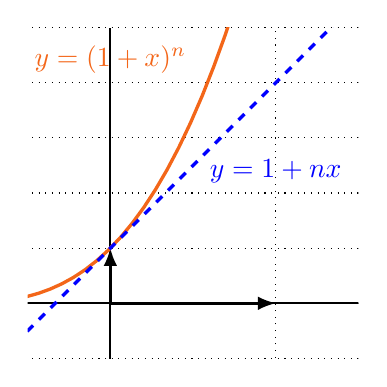
\begin{tikzpicture}[scale=0.7,x={(3cm,0cm)},y={(0cm,1cm)}]
\clip (-0.5,-1) rectangle (1.5,5);
\draw [thin, dotted] (-2,-4) grid[xstep=1,ystep=1] (6,7);
\draw [thick] (-4,0)--(7,0);
\draw [thick] (0,-4) -- (0,5);
\draw [very thick,->,>=latex] (0,0)--(0,1);
\draw [very thick,->,>=latex] (0,0)--(1,0);
\draw [very thick, ocre,domain=-1:6,samples=100] plot (\x,{(1+\x)^3});
\draw [very thick, blue, dashed,domain=-1:6] plot (\x,1+3*\x);
\draw [blue] (1,2) node[above] {$y=1+nx$};
\draw [ocre] (0,4) node[above] {$y=(1+x)^n$};
\end{tikzpicture}
\end{center}\end{minipage}\hfill
\begin{minipage}{0.65\linewidth}
Une interprétation graphique de cette inégalité est possible.

La droite d'équation $y=1+nx$ n'est autre que la tangente à la courbe d'équation $y=(1+x)^n$ à l'abscisse 0. L'inégalité de Bernoulli dit donc que la courbe se trouve au-dessus de la tangente lorsque $x>0$.
\vskip5pt
Nous verrons, lorsque la dérivation n'aura plus de secret pour vous, que cette remarque nous fournira une autre démonstration de l'inégalité de Bernoulli.
\end{minipage}



\section{Suites majorées, minorées, bornées}

\begin{definition}[Suites majorées, minorées, bornées] Soit $(u_n)$ une suite réelle. On dit que...
\begin{itemize}
\item ...$(u_n)$ est \textit{majorée} s'il existe un réel $M$ tel que, pour tout entier naturel $n$, $u_n \leqslant M$.\\ Un tel réel $M$ est alors appelé \textit{majorant} de la suite $(u_n)$.
\vskip5pt
\item ...$(u_n)$ est \textit{minorée} s'il existe un réel $m$ tel que, pour tout entier naturel $n$, $u_n \geqslant m$.\\ Un tel réel $m$ est alors appelé \textit{minorant} de la suite $(u_n)$.
\vskip5pt
\item ...$(u_n)$ est \textit{bornée} si $(u_n)$ est à la fois majorée et minorée.
\end{itemize}\end{definition}

Les majorants et minorants sont indépendants de $n$ ! Bien que pour tout $n>0$, on ait $n \leqslant n^2$, on ne peut pas dire que la suite $(u_n)$ définie par $u_n=n$ est majorée. Cette indépendance se traduit dans l'ordre des quantificateurs employés dans la définition précédente (le majorant y apparaît avant l'entier $n$).


\begin{example}Pour tout $n$, on pose $u_n=\cos (n)$. 

La suite $(u_n)$ est bornée puisque, pour tout entier $n$, $-1 \leqslant u_n \leqslant 1$.\end{example}

\begin{example} Pour tout entier naturel $n$, on pose $v_n=n^2+1$. La suite $(v_n)$ est minorée puisque pour tout entier naturel $n$, $v_n\geqslant 1$. En revanche, elle n'est pas majorée. \end{example}

\begin{example} Pour tout entier naturel $n$, on pose $w_n=(-1)^n \, n$. Cette suite n'est ni majorée, ni minorée.\end{example}

Lorsqu'une suite est définie par récurrence, une majoration ou une minoration de cette suite peut elle-même être démontrée par récurrence.

\begin{example} On considère la suite $(u_n)$ définie par $u_0 = 5$ et pour tout entier naturel $n$, $u_{n+1}=0.5u_n + 2$. Pour tout entier naturel $n$, on note $\mathcal{P}(n)$ la proposition « $u_n \geqslant 4$ ».
\begin{itemize}
\item \textbf{Initialisation} : On a bien $u_0 \geqslant 4$. $\mathcal{P}(0)$ est donc vraie.
\vskip5pt
\item \textbf{Hérédité} : Soit $n\in\mathbb{N}$. Supposons que $\mathcal{P}(n)$ est vraie, c'est-à-dire $u_n \geqslant 4$. 

En multipliant cette inégalité par $0,5$, on en déduit que $0,5 u_n \geqslant 2$. 

En ajoutant 2, on en déduit que $0,5u_n+2 \geqslant 4$, c'est-à-dire $u_{n+1}\geqslant 4$. 

$\mathcal{P}(n+1)$ est donc vraie.
\vskip5pt
\item \textbf{Conclusion :} Ainsi, $\mathcal{P}(0)$ est vraie et la proposition $\mathcal{P}$ est héréditaire. 

D'après le principe de récurrence, on en conclut que pour tout entier naturel $n$, $\mathcal{P}(n)$ est vraie.
\end{itemize}\end{example}

\newpage

Si l'on se donne une fonction $f$ définie sur un ensemble $I$ et une suite $(u_n)$ à valeurs dans $I$ telle que, pour tout entier naturel $n$, $u_{n+1}=f(u_n)$, l'étude de la fonction $f$ pourra également nous fournir des informations sur la suite $(u_n)$ étudiée.

\begin{example}On considère une fonction $f$ définie sur $\mathbb{R}$ et dont le tableau de variations est le suivant.

\begin{center}
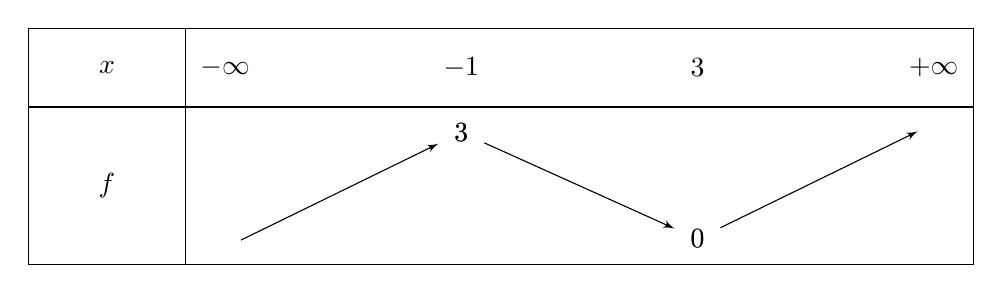
\begin{tikzpicture}[scale=1]
\tikzset{node style/.style = {inner sep = 2pt, outer sep = 2pt}}
   \tkzTabInit{$x$ / 1 , $f$ / 2}{$-\infty$, $-1$, $3$,$+\infty$}
   \tkzTabVar{-/$ $,+/$3$,-/$0$,+/$ $}
\end{tikzpicture}\end{center}

On considère alors la suite $(u_n)$ définie par $u_0=1$ et, pour tout entier naturel $n$, $u_{n+1}=f(u_n)$. 

Pour tout entier naturel $n$, on considère la proposition $\mathcal{P}(n)$ : « $0 \leqslant u_n \leqslant 3$ ».
\begin{itemize}
\item \textbf{Initialisation} : On a bien $0 \leqslant u_0 \leqslant 3$. $\mathcal{P}(0)$ est donc vraie.
\vskip5pt
\item \textbf{Hérédité} : Soit $n\in\mathbb{N}$. Supposons que $\mathcal{P}(n)$ est vraie, c'est-à-dire $0 \leqslant u_n \leqslant 3$. 

La fonction $f$ est décroissante sur l'intervalle $[-1;3]$, lequel contient l'intervalle $[0;3]$. Il est alors possible d'appliquer cette fonction à notre inégalité (attention, la fonction étant décroissante, l'inégalité sera alors renversée).

Ainsi, on a $f(0) \geqslant f(u_n) \geqslant f(3)$. On sait par ailleurs que $f(u_n)=u_{n+1}$ et que $f(3)=0$.

Enfin, d'après les variations de $f$, on sait également que $f(-1) \geqslant f(0)$, c'est-à-dire que $3 \geqslant f(0)$.

Ainsi, $3 \geqslant f(0) \geqslant f(u_n) \geqslant f(3)$, c'est-à-dire $3\geqslant f(0) \geqslant u_{n+1} \geqslant 0$.

On en conclut en particulier que $3 \geqslant u_{n+1} \geqslant 0$. $\mathcal{P}(n+1)$ est donc vraie.
\vskip5pt
\item \textbf{Conclusion} : Ainsi, $\mathcal{P}(0)$ est vraie et la proposition $\mathcal{P}$ est héréditaire. D'après le principe de récurrence, on en conclut que pour tout entier naturel $n$, $\mathcal{P}(n)$ est vraie.
\end{itemize}\end{example}



\section{Suites croissantes, suites décroissantes}

\begin{definition}[Variations d'une suite]Soit $(u_n)$ une suite réelle et $n_0$ un entier naturel.

\begin{itemize}
\item On dit que $(u_n)$ est \textit{croissante} à partir de $n_0$ si, pour tout entier naturel $n\geqslant n_0$, $u_{n+1} \geqslant u_n$.
\vskip5pt
\item On dit que $(u_n)$ est \textit{décroissante} à partir de $n_0$ si, pour tout entier naturel $n\geqslant n_0$, $u_{n+1} \leqslant u_n$.
\end{itemize}\end{definition}

Étudier la croissance ou la décroissance d'une suite revient donc souvent à étudier le signe de $u_{n+1}-u_n$.

\begin{example}On considère la suite $(u_n)$ définie pour tout entier naturel $n$ par $u_n=n^2-n$. 

Pour tout entier naturel $n$,
\[u_{n+1}-u_n = (n+1)^2-(n+1)-(n^2-n)=n^2+2n+1-n-1-n^2-1=2n \geqslant 0.\]
La suite $(u_n)$ est donc croissante.\end{example}
\newpage
\begin{proposition}Soit $(u_n)$ une suite \textbf{strictement positive} et $n_0$ un entier naturel. 
\begin{itemize}
\item $(u_n)$ est croissante à partir de $n_0$ si, pour tout entier naturel $n\geqslant n_0$, $\dfrac{u_{n+1}}{u_n} \geqslant 1$.
\vskip5pt
\item $(u_n)$ est décroissante à partir de $n_0$ si, pour tout entier naturel $n\geqslant n_0$, $\dfrac{u_{n+1}}{u_n} \leqslant 1$.
\end{itemize}
\end{proposition}

\begin{example}On considère la suite $(u_n)$ définie pour tout entier naturel non nul $n$ par $u_n=\dfrac{2^n}{n}$. 

Pour tout entier naturel non nul $n$, on a $u_n>0$ et 
\[\dfrac{u_{n+1}}{u_n}=\dfrac{\dfrac{2^{n+1}}{n+1}}{\dfrac{2^n}{n}}=\dfrac{2^{n+1}}{n+1}\times \dfrac{n}{2^n} = \dfrac{2n}{n+1}.\]
Or, si $n\geqslant 1$, on a, en ajoutant $n$ aux deux membres de l'inégalité, $2n \geqslant n+1$ et donc $\dfrac{2n}{n+1}\geqslant 1$. \\ Ainsi, pour tout entier naturel non nul $n$, $\dfrac{u_{n+1}}{u_n}\geqslant 1$. La suite $(u_n)$ est donc croissante.\end{example}

Encore une fois, lorsqu'une suite est définie par récurrence, ses variations peuvent également être étudiées par récurrence.

\begin{example}On considère la suite $(u_n)$ définie par $u_0=4$ et pour tout $n\in\mathbb{N}$, $u_{n+1}=\sqrt{5+u_n}$.

Pour tout entier naturel $n$, on note $\mathcal{P}(n)$ la proposition $0\leqslant u_{n+1} \leqslant u_n$. Montrer que $\mathcal{P}(n)$ est vraie pour tout entier naturel $n$ démontrera que la suite $(u_n)$ est décroissante et minorée par 0, un résultat qui nous intéressera fortement dans un prochain chapitre...

\begin{itemize}
\item \textbf{Initialisation :} $u_0=4$, $u_1=\sqrt{5+4}=\sqrt{9}=3$. On a bien $0 \leqslant u_1 \leqslant u_0$. $\mathcal{P}(0)$ est vraie.
\vskip5pt
\item \textbf{Hérédité :} Soit $n\in\mathbb{N}$. Supposons que $\mathcal{P}(n)$ est vraie. On a alors
\[0\leqslant u_{n+1} \leqslant u_n.\]
En ajoutant 5 à chaque membre, on obtient
\[5\leqslant u_{n+1} +5\leqslant u_n+5.\]
On souhaite "appliquer la racine carrée" à cette inégalité. La fonction $x\mapsto \sqrt{x}$ étant croissante sur l'intervalle $[0;+\infty[$, l'appliquer ne changera pas le sens de l'inégalité. On a donc bien
\[ \sqrt{5} \leqslant \sqrt{u_{n+1}+5} \leqslant \sqrt{u_n+5}.\]
D'une part, $\sqrt{5} \geqslant 0$. D'autre part, $\sqrt{u_{n+1}+5}=u_{n+2}$ et $\sqrt{u_{n}+5}=u_{n+1}$. Ainsi,
\[0 \leqslant u_{n+2} \leqslant u_{n+1}.\]
La proposition $\mathcal{P}(n+1)$ est donc vraie.
\vskip5pt
\item \textbf{Conclusion :} $\mathcal{P}(0)$ est vraie et $\mathcal{P}$ est héréditaire. Par récurrence, $\mathcal{P}(n)$ est vraie pour tout $n\in\mathbb{N}$.

\end{itemize}\end{example}
\newpage
Comme précédemment, si l'on dispose d'une fonction $f$ que l'on sait étudier et d'une suite $(u_n)$ telle que pour tout entier naturel $n$, $u_{n+1}=f(u_n)$, il est sans doute possible d'utiliser les informations que nous avons sur la fonction pour en déduire des informations sur notre suite.

\textbf{Attention ! Ce n'est pas parce que la fonction $f$ est croissante que la suite le sera également !}


\begin{example}On considère une fonction $f$ définie sur $\mathbb{R}$ et dont le tableau de variations est le suivant.

\begin{center}
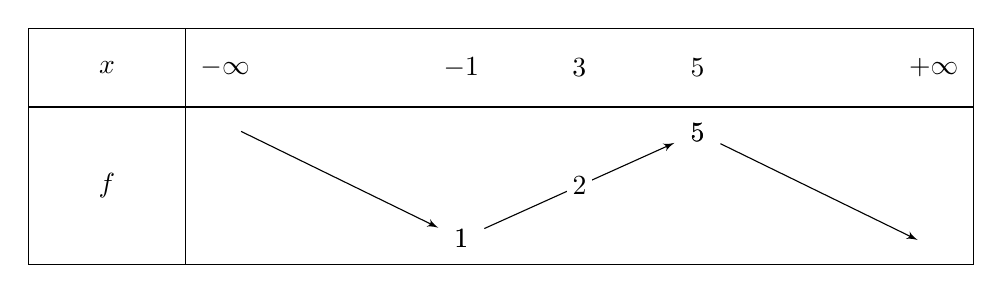
\begin{tikzpicture}[scale=1]
\tikzset{node style/.style = {inner sep = 2pt, outer sep = 2pt}}
   \tkzTabInit{$x$ / 1 , $f$ / 2}{$-\infty$, $-1$, $5$,$+\infty$}
   \tkzTabVar{+/$ $,-/$1$,+/$5$,-/$ $}
   \tkzTabVal{2}{3}{0.5}{$3$}{$2$}
\end{tikzpicture}\end{center}

On considère alors la suite $(u_n)$ définie par $u_0=3$ et, pour tout entier naturel $n$, $u_{n+1}=f(u_n)$. 

On souhaite montrer que la suite $(u_n)$ est décroissante et bornée par $-1$ et $5$. Pour tout entier naturel $n$, on considère alors la proposition $\mathcal{P}(n)$ : « $-1 \leqslant u_{n+1} \leqslant u_n \leqslant 5$ ».
\begin{itemize}
\item \textbf{Initialisation} : On a $u_0=3$ et $u_1=f(u_0)=f(3)=2$. On a bien $-1 \leqslant u_1 \leqslant u_0 \leqslant 5$. $\mathcal{P}(0)$ est donc vraie.
\vskip5pt
\item \textbf{Hérédité} : Soit $n\in\mathbb{N}$. Supposons que $\mathcal{P}(n)$ est vraie, c'est-à-dire $-1 \leqslant u_{n+1} \leqslant u_n \leqslant 5$. 

La fonction $f$ est croissante sur l'intervalle $[-1;5]$. Il est alors possible d'appliquer cette fonction à notre inégalité (la fonction étant croissante, le sens de l'inégalité est conservée).

Ainsi, on a $f(-1) \leqslant f(u_{n+1}) \leqslant f(u_n) \leqslant f(5)$. 

On sait par ailleurs que $f(u_n)=u_{n+1}$, que $f(u_{n+1})=u_{n+2}$, que $f(5)=5$ et enfin que $f(-1)=1\geqslant -1$.

On en conclut donc que $-1 \leqslant u_{n+1} \leqslant u_n \leqslant 5$. $\mathcal{P}(n+1)$ est donc vraie.
\vskip5pt
\item \textbf{Conclusion} : Ainsi, $\mathcal{P}(0)$ est vraie et la proposition $\mathcal{P}$ est héréditaire. D'après le principe de récurrence, on en conclut que pour tout entier naturel $n$, $\mathcal{P}(n)$ est vraie.
\end{itemize}\end{example}







\end{document}